\documentclass[compress]{beamer}
%--------------------------------------------------------------------------
% Common packages
%--------------------------------------------------------------------------
\usepackage[T1]{fontenc}
\usepackage{graphicx}
\usepackage{multicol}
\usepackage{tabularx,ragged2e}
\usepackage{booktabs}
\usepackage{listings}
\lstset{ %
language=erlang,
basicstyle=\normalsize\ttfamily,
keywordstyle=,
numbers=left,
numberstyle=\tiny\ttfamily,
stepnumber=1,
showspaces=false,
showstringspaces=false,
showtabs=false,
breaklines=true,
frame=tb,
framerule=0.5pt,
tabsize=4,
framexleftmargin=0.5em,
framexrightmargin=0.5em,
xleftmargin=0.5em,
xrightmargin=0.5em
}

%--------------------------------------------------------------------------
% Load theme
%--------------------------------------------------------------------------
\usetheme{hsrm}

\usepackage{tikz}
\usetikzlibrary{mindmap,backgrounds}

%--------------------------------------------------------------------------
% General presentation settings
%--------------------------------------------------------------------------
\title{Functional Algebra by Example}
\date{Last Updated: \today}
\author{Susan Potter \small{@SusanPotter}}

%--------------------------------------------------------------------------
% Notes settings
%--------------------------------------------------------------------------
%\setbeameroption{show notes}

\begin{document}
%--------------------------------------------------------------------------
% Titlepage
%--------------------------------------------------------------------------

\maketitle

%--------------------------------------------------------------------------
% Table of contents & whoami
%--------------------------------------------------------------------------
%\section*{Outline}
%\begin{frame}{Outline}
%  \tableofcontents[hideallsubsections]
%\end{frame}

\begin{frame}{whoami}
  \begin{figure}
    \centering
    \includegraphics[width=0.55\textwidth]{assets/trust_me_panda.jpg}
  \end{figure}
  \note<1>{An app + middleware dev who has felt Ops pain too}
\end{frame}

%--------------------------------------------------------------------------
% Content
%--------------------------------------------------------------------------
\section{Background}

\begin{frame}{Model/Assumptions}
  \begin{figure}
    \includegraphics[width=0.8\textwidth]{assets/model.jpg}
  \end{figure}
\end{frame}

\begin{frame}{Motivating Uses}
  \begin{figure}
    \includegraphics[width=0.8\textwidth]{assets/motivating_uses.jpg}
  \end{figure}
\end{frame}

\begin{frame}{Common Approaches}
  \begin{figure}
    \includegraphics[width=0.8\textwidth]{assets/common_approaches.jpg}
  \end{figure}
\end{frame}

\begin{frame}{Why Distribute? Why Decentralize?}
  \begin{itemize}
    \item \Large{Probability of system failure}
    \item \Large{Large datasets (data locality)}
    \item \Large{Eliminate SPOFs}
    \item \Large{Commodity hardware}
  \end{itemize}
\end{frame}

\begin{frame}
  \begin{figure}
    \centering
    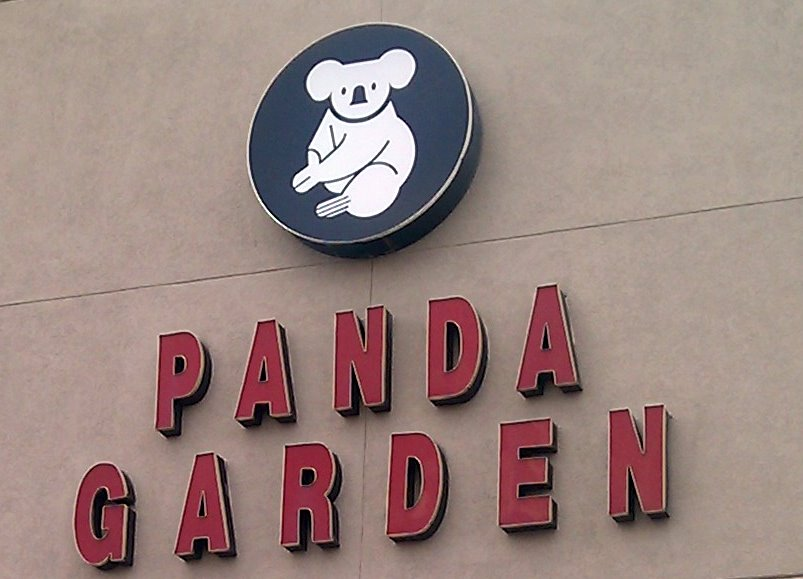
\includegraphics[width=\linewidth]{assets/panda_garden_fail.jpg}
  \end{figure}
\end{frame}

\section{Concepts \& Intuitions}

\begin{frame}{Layers}
  \begin{figure}
    \centering
    \includegraphics[width=\linewidth]{assets/layers.jpg}
  \end{figure}
\end{frame}

\begin{frame}{Terminology (core)}
\begin{itemize}
  \item Partition
  \item Vnode
  \item Hinted Handoff
  \item Read Repair
\end{itemize}
\end{frame}

\begin{frame}{Terminology (pipe)}
\begin{itemize}
  \item Pipe
  \item Fitting ("phase")
  \item Queue
  \item Worker
\end{itemize}
\end{frame}

\begin{frame}[containsverbatim]{Example UNIX Pipe}
\begin{lstlisting}[language=bash]
find . -name "*.rb" \
  | xargs egrep "#.*?TODO:" \
  | wc -l
\end{lstlisting}
  \small{Character-based, through file descriptors}
\end{frame}

\begin{frame}[containsverbatim]{Example Function Composition}
\begin{lstlisting}[language=haskell]
(length . mapToUpper . sanitize) input
\end{lstlisting}
  \small{Value based, through functions}
\end{frame}

\begin{frame}[containsverbatim]{Example Riak Pipe}
\begin{lstlisting}[language=erlang]
[ #fitting_spec{ name=fetch_trades
               , module=riskmgr_fetch_trades
               , ...}
, #fitting_spec{ name=calc_var
               , module=riskmgr_calc_var
               , ...}
]
\end{lstlisting}
  \small{Message-based, across nodes}
\end{frame}

\begin{frame}{vnode and workers}
  \begin{itemize}
    \item \Large{vnode} \newline \small{manages lifecycle and queues of workers} \newline
    \item \Large{vnode worker} \newline \small{processes inputs}
  \end{itemize}
\end{frame}

\begin{frame}[containsverbatim]{vnode worker behavior}
\begin{lstlisting}
behaviour_info(callbacks) ->
    [{init,2},
     {process,3},
     {done,1}];
behaviour_info(_Other) ->
    undefined.
%% Optionally two more too, not required.
\end{lstlisting}
\end{frame}

\begin{frame}{Distribution: \tt{chashfun}}
\begin{itemize}
  \item Use random uniform hash fun to saturate workers
  \item See Bryan Fink's previous Pipe presentations
\end{itemize}
\end{frame}

\begin{frame}[containsverbatim]{Validation}
\begin{lstlisting}
% #fitting_spec { module = ..., arg = 43, ... }
% validate_arg/1
validate_arg(Arg) when is_integer(Arg) -> ok;
validate_arg(Arg) when is_atom(Arg) -> ok;
validate_arg(_) -> {error, "Argument must be a valid integer or atom"}.
\end{lstlisting}
\end{frame}

\begin{frame}{Leaky Pipes}
  \begin{figure}
    \centering
    \includegraphics[width=0.55\textwidth]{assets/leaky_pipe.jpg}
  \end{figure}
  \small{http://www.flickr.com/photos/thirteenofclubs/}
\end{frame}

\begin{frame}[containsverbatim]{Riak (Core) Mechanics}
\begin{itemize}
  \item \Large{Handoff} \newline \small{Migrate vnodes from node to node}
\end{itemize}
\begin{lstlisting}
% Old Node
% Called with last known State of worker
archive/1 % returns {ok, Archive}

% New Node
% Called with Archive and State from old node
handoff/2 % returns {ok, NewState}
\end{lstlisting}
\end{frame}

\begin{frame}{Failures}
  \begin{itemize}
    \item{\Large{validate\_arg} \newline \small{Seen above}}
    \item{\Large{Pipe client process dies} \newline \small{YOLO}}
    \item{\Large{nval} \newline \small{How many vnodes to ask before failing, default 1}}
    \item{\Large{vnode worker logic} \newline \small{Think using dataflow semantics}}
  \end{itemize}
\end{frame}

\begin{frame}{Existing Fittings}
  \begin{itemize}
    \item{\Large{\tt{riak\_pipe\_w\_tee}} \newline \small{Useful for intermediate results}} \newline
    \item{\Large{\tt{riak\_pipe\_w\_xform}} \newline \small{Simple delegater: 3-arity function}} \newline
    \item{\Large{\tt{riak\_pipe\_w\_reduce}} \newline \small{What you would expect: simple accumulating reduce}} \newline
    \item{\Large{\tt{riak\_kv\_pipe\_get}} \newline \small{Take advantage of data locality with cohosted KV store}}
  \end{itemize}
\end{frame}

\section{Applications}

\begin{frame}{Known Uses}
\begin{itemize}
  \item \Large{Riak's Map/Reduce}
  \item \Large{Risk metrics}
  \item \Large{Tenant Usage}
\end{itemize}
\end{frame}

\begin{frame}{Troubleshooting}
  \begin{itemize}
    \item{\Large{\tt{riak\_pipe:status/1}} \newline \small{Provides fittings, processed, failures, queue\_length, etc stats}}
    \item{\Large{\tt{riak\_pipe\_w\_crash} fitting} \newline \small{Used to test Riak Pipe}}
    \item{\Large{\tt{riak\_pipe:active\_pipelines/1}} \newline \small{See all active pipelines}}
    \item{\Large{\tt{riak\_pipe\_cinfo module}} \newline \small{cluster info interrogation module}}
  \end{itemize}
\end{frame}

\begin{frame}{Further Work}
  \begin{itemize}
    \item More applications (e.g. genetics, 3rd party APIs with rate limits)
    \item Decentralized pipe control
    \item Measure "completeness" of resultset
  \end{itemize}
\end{frame}

\begin{frame}{Related Work}
  \begin{itemize}
    \item "Pipe" libraries EVERYWHERE (pipe, scalaz-stream)
    \item riak\_pg
    \item Map-Reduce frameworks
    \item Staged Event Driven Architecture
    \item Event Stream Processing
    \item Dataflow multi-stage processing
  \end{itemize}
\end{frame}

\begin{frame}{Royal Fail}
  \begin{figure}
    \centering
    
\includegraphics[width=0.5\textwidth]{assets/royal_fail.jpg}
  \end{figure}
  \small{http://www.flickr.com/photos/dadavidov/}
\end{frame}

\begin{frame}{Questions}
  \begin{figure}
    \centering
    
\includegraphics[width=0.5\textwidth]{assets/royal_fail.jpg}
  \end{figure}
  \Large{Questions?}
\end{frame}

\end{document}
